\documentclass[a4paper]{article}

\usepackage{fullpage} % Package to use full page
\usepackage{parskip} % Package to tweak paragraph skipping
\usepackage{tikz} % Package for drawing
\usepackage{amsmath}
\usepackage{hyperref}
\usepackage{enumerate}
\usepackage{graphicx}
\usepackage{booktabs}
\title{Midterm 02}
\author{Jeff Tilton}
\date{November, 25 2019}

\begin{document}

\maketitle

\section{Boosting Algorithms}
\begin{enumerate}[(a)]
\item Explain the weights $D_2(i)$ for each sample after the first iteration. You can explain by drawing figures similar to what we have in class.

Incorrect classifications are boosted after each iteration in adaboost.  This allows these incorrect classifications to become more important in subsequent iterations.  In our current example only one item was missclassified.  Therefore this point will have a higher weight than the other points in the subsequent iteration.  Weights are determined by 

$$\frac{D_t(i)}{Z_t}x 
\begin{cases}  e^{-\alpha_t} & \text{if } y_i=h_t(x_i) \\
			   e^{\alpha_t} & \text{if } y_i \neq h_t(x_i)
\end{cases}
$$

From the above equation we can see that the algorithm boosts incorrect classifications by giving adding weight to the incorrectly classified items and subtracting weight from the correctly classified items.



\item Calculate the weight $\alpha_1$ assigned to $h_1$ by Adaboost.

$$
\alpha_t = \frac{1}{2} ln \left( \frac{1-\epsilon_t}{\epsilon_t} \right) >0
$$

$h_1$ stump miscalculated 1 item.  Therefore $\epsilon = 1/8$.  Plugging in the numbers we get $\alpha = 0.97$

\item True/False (5 points) The votes $\alpha_i$ assigned to weak classifiers in boosting generally goes down as the algorithm proceeds, because the weighted training error of the weak classifiers tend tends to go up.

False

\item True/False (5 points) The votes $\alpha$ assigned to the classifiers assembled by Adaboost are always non-negative.

True this can be seen in the equation for $\alpha$ above.

\end{enumerate}

\section{Random forrest for email spam classifier}
\begin{enumerate}
\item (5 points) Load the data from spambase.data. If there are missing values, you can just fill in zero. Report: How many instances and how many features for each instance in the data set? How many instances of spam versus regular emails are there in the data?


There are a total of 4601 samples and 57 features.  Of those samples there are total of 1,813 spam emails.  

\item Choose an appropriate depth of the tree, report the accuracy and the tree model fitted, similar to what is shown on Page 16 of “Random forest” lecture. In Python, this can be done export graphviz which output a dot file.

I chose a depth of 8 and had an accuracy of.92.  The resulting split is seen below. 

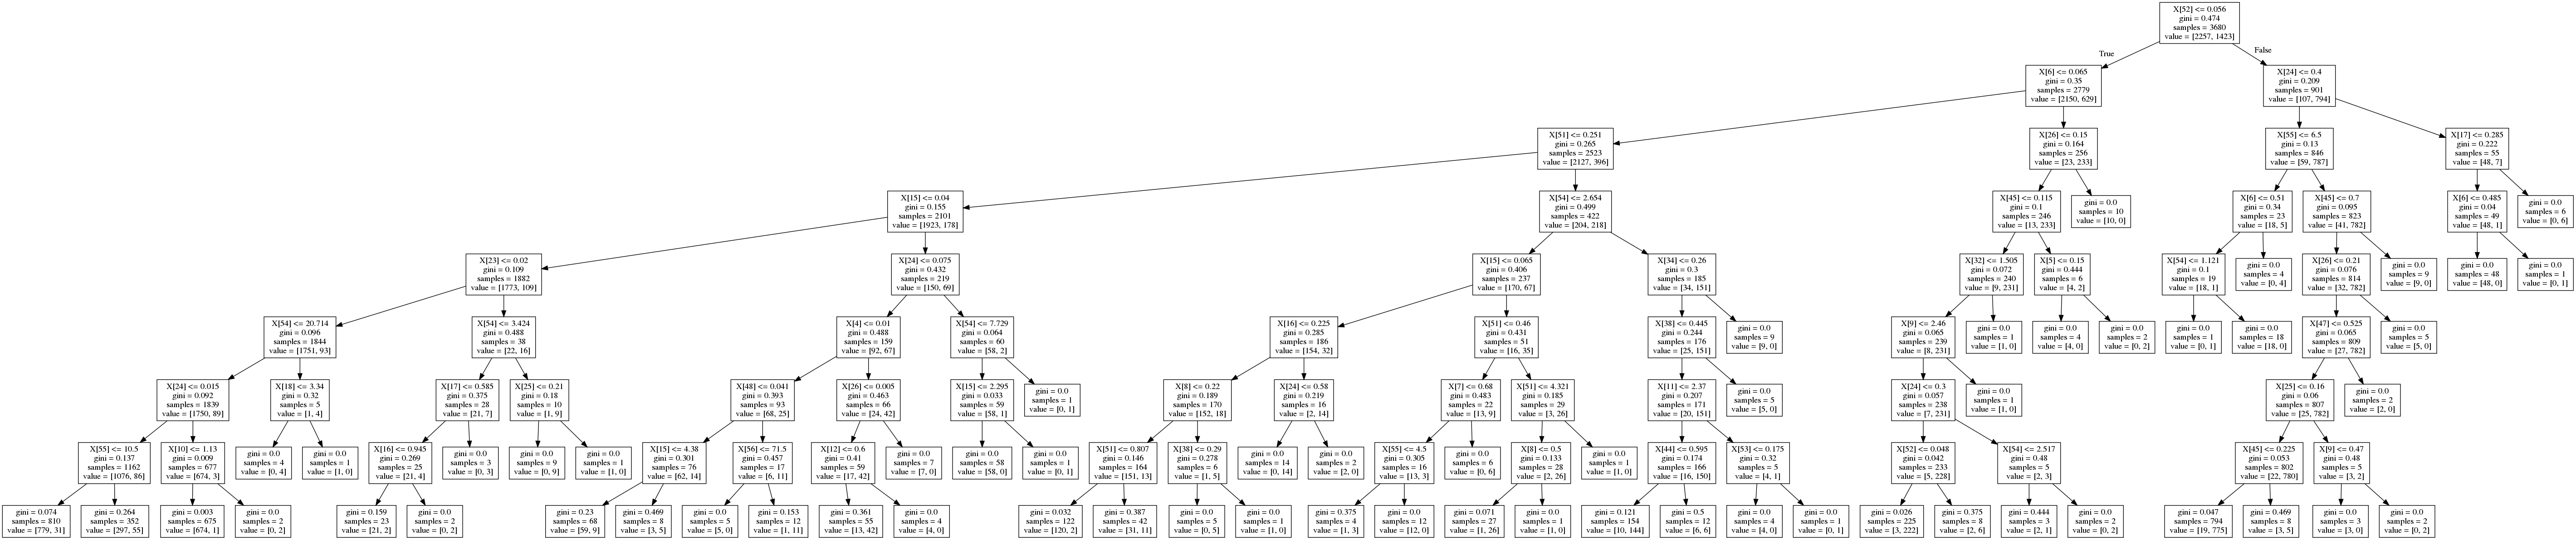
\includegraphics[width=\textwidth]{tree.png}

\item Build a random forest model.  Report the accuracy and classifier structure similar as decision tree classifier above.

I used a random grid search to determine the best max depth and number of trees to use in the forest.  I came up with a max depth of 17 and 121 trees to reach an accuracy of .95.

\item Compare and report the AUC for your classification tree and random forest models on testing data, respectively.

The AUC scores for the tree classifier and random forest classifier are seen in the table below.

\begin{center}
\begin{tabular}{ |c|c|c|c| } 
\hline
Tree & Random Forest\\
\hline
.91 & .95 \\ 
\hline
\end{tabular}
\end{center}



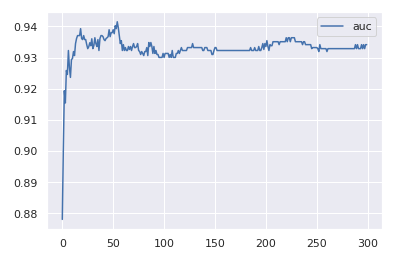
\includegraphics[width=\textwidth]{auc.png}



\end{enumerate}
\section{Nonlinear regression and cross-validation}

The coefficient of thermal expansion y changes with temperature x. An experiment to relate
y to x was done. Temperature was measured in degrees Kelvin. (The Kelvin temperature is
the Celcius temperature plus 273.15). The raw data file is copper-new.txt.

\begin{enumerate}
\item Perform linear regression on the data. Report the fitted model and the fitting error.

Linear regression model attributes are as follows:
\begin{enumerate}[]
  \item Mean squared error: 10.52
  \item Coefficient: 0.021
  \item Intercept: 1.57
  \item $\text{R}^2$: 0.686
\end{enumerate}

\item Perform nonlinear regression with polynomial regression function up to
degree n = 10 and use ridge regression (see Lecture Slides for “Bias-Variance Trade-
off”). Write down your formulation and strategy for doing this, the form of the ridge
regression.

I chose a single lambda value ($\lambda = 100$) and performed polynomial ridge regression from degree 1:10.

The reults are as follows:

\begin{tabular}{lrrr}

degree &    R\textasciicircum 2 &     mse \\

1 &  0.686 &  10.521 \\
2 &  0.878 &   4.093 \\
3 &  0.968 &   1.085 \\
4 &  0.993 &   0.220 \\
5 &  0.998 &   0.069 \\
6 &  0.998 &   0.072 \\
7 &  0.998 &   0.058 \\
8 &  0.998 &   0.057 \\
9 &  0.999 &   0.042 \\
10 &  0.999 &   0.027 \\

\end{tabular}

\item Use 5 fold cross validation to select the optimal regularization parameter
$\lambda$. Plot the cross validation curve and report the optimal $\lambda$.

For this exercise I used sklearn's RidgeCV method to determine the best lambda between 0:200 for each polynomial 1:10.  I then used cross validation for each polynomial's best lambda to come up with a mean squared error score for each polynomial.  I determined that polynomial 5 with $\lambda=0.85$ was the best model having a mean squared error of 0.09.

The cross validation curve for the chosen model can be seen below.  

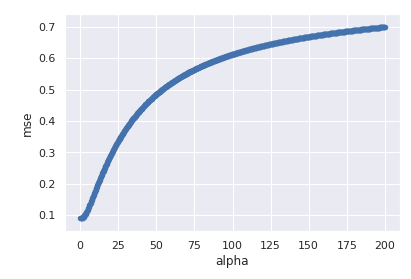
\includegraphics[width=\textwidth]{cv.png}

The bias variance tradeoff can be seen in the next plot, which is the log(mse) of a given polynomial with it's best $\lambda$ value found by cross validation.  

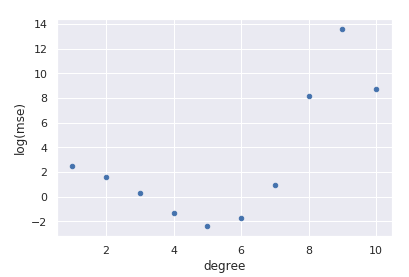
\includegraphics[width=\textwidth]{bv.png}

\item Predict the coefficient at 400 degree Kelvin using both models. Comment
on how would you compare the accuracy of predictions.

Model 1 (linear regression) and model 2 (Ridge regression $degree=5, \alpha=0.85$) predictions for the thermal coefficient of expansion are shown in the table below.

\begin{tabular}{lrr}
\toprule
Model 1 &  Model 2 \\
\midrule
10.08 &    12.12 \\
\bottomrule
\end{tabular}

I linearly interpolated at 400 to get a value of 12.5.  Although this is not a true measure of accuracy it can give me a pretty good indication of which model has done a better prediction at 400.  The linear regression model is off by an absolute value of 2.42 where the ridge regression model is off by an absolute value of 0.38.  Therefore the ridge regression model does a better job of predicting the coefficient at 400 degrees kelvin.

\end{enumerate}
\end{document}